%
% $Id$ 
%
% $LastChangedDate$ 
% 
% $LastChangedBy$
%

\documentclass[10pt]{report}
\usepackage{graphicx}
\usepackage{setspace}			
\onehalfspacing
% numbering down to subsubsection
\setcounter{secnumdepth}{3}

\title{CS6999 Web Data and Text Mining:\\Parallel Text Indexer Project Report}
\author{Damien DuBios\\Justin Kamerman 3335272\\Raman Singh}
\date{\today}

\begin{document}
\maketitle
% No chapter numbers
\renewcommand*\thesection{\arabic{section}}

%----------------------------------------
% Introduction
%----------------------------------------
\section{Introduction}
Briefly in at most one page describe the main idea of the project and why is it important\\

%----------------------------------------
% Literature Review
%----------------------------------------
\section{Literature Review}
\label{sec:literaturereview}
The Aho-Corasick string matching algorithm\cite{RefWorks:103} is a
kind of dictionary matching search algorithm that constructs a finite
state machine to scan for a given set of keywords. It is, in effect, a
reduced grammar regular expression parser described in
\cite{RefWorks:111}. In our search implementation, the finite state
machine is constructed from a list of keywords. Then the documents
of the test corpus are read from secondary storage and fed through the
finite state machine. As soon as a document is found to contain at
least one instance of each of a set of search terms, parsing of that document
ends.


%----------------------------------------
% Motivation
%----------------------------------------
\section{Motivation}
\label{sec:motivation}


%----------------------------------------
% Research Plan
%----------------------------------------
\section{Research Plan}
\label{sec:researchplan}


%----------------------------------------
% Design Component
%----------------------------------------
\section{Design Component}
\label{sec:designcomponent}
A black-box functional view of the indexing system is show in figure
\ref{fig:blackbox}. The system proceses a continuous incoming flow of
documents and distribute them to parallel indexing threads running on
physically seprate, heterogenous nodes.  Document queries are performed
using an evolving search index. The operational balance is to
timeously index new additions to the corpus while servicing concurrent
search requests. A view as to how the components of the indexer system
are deployed is show in figure \ref{fig:deploymentmodel}.

As can be seen in figure \ref{fig:deploymentmodel}, the indexer
processes are symmetrical and deployed on muliple physical nodes. The
individual indexers do not interact directly with one another, making
for a simple deployment and operation model. The execution loop of
each indexer is as follows:

\begin{enumerate}
\item Initialize the indexer by retrieving a collection of index
  keywords and synonyms from a relational databse. These keywords are
  used to construct a lexical parser which will be used to scan and
  index documents.
\item Retrieve a batch of unprocessed documents from a relational
  database. The document batch will be sized according to the physical
  capabilities of each node. In this implementation, this tuning task
  is a manual exercise but future enhancements may include an adaptive
  loading component.
\item Parse each document retrieved and contruct an inverted index
  representing the batch. This \textit{delta} index, as we shall call
  it, is then used to augment the global index maintained in a
  relational database.
\item Repeat from step 2.
\end{enumerate}

As shown in figure \ref{fig:deploymentmodel}, the searcher component
can be executed from any node which has access to the relational
database housing the document index. The execution path of a single
search query wold be as follows:

\begin{enumerate}
  \item Canonize search terms based on keyword synonyms defined in the
    keyword store.
  \item Execute a boolean query against the inverted index.
  \item Return the list of corpus documents containing the
    intersection of the canons of the search terms.
\end{enumerate}

\begin{figure}
  \begin{center}
	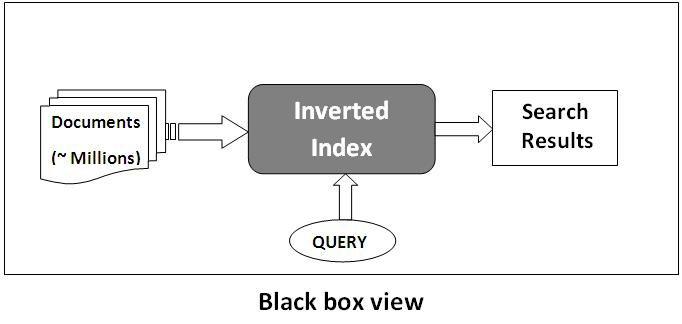
\includegraphics[width=\textwidth,height=!]{blackbox}
  \end{center}
  \caption{A black-box view of the indexer}
  \label{fig:blackbox}
\end{figure} 


\begin{figure}
  \begin{center}
	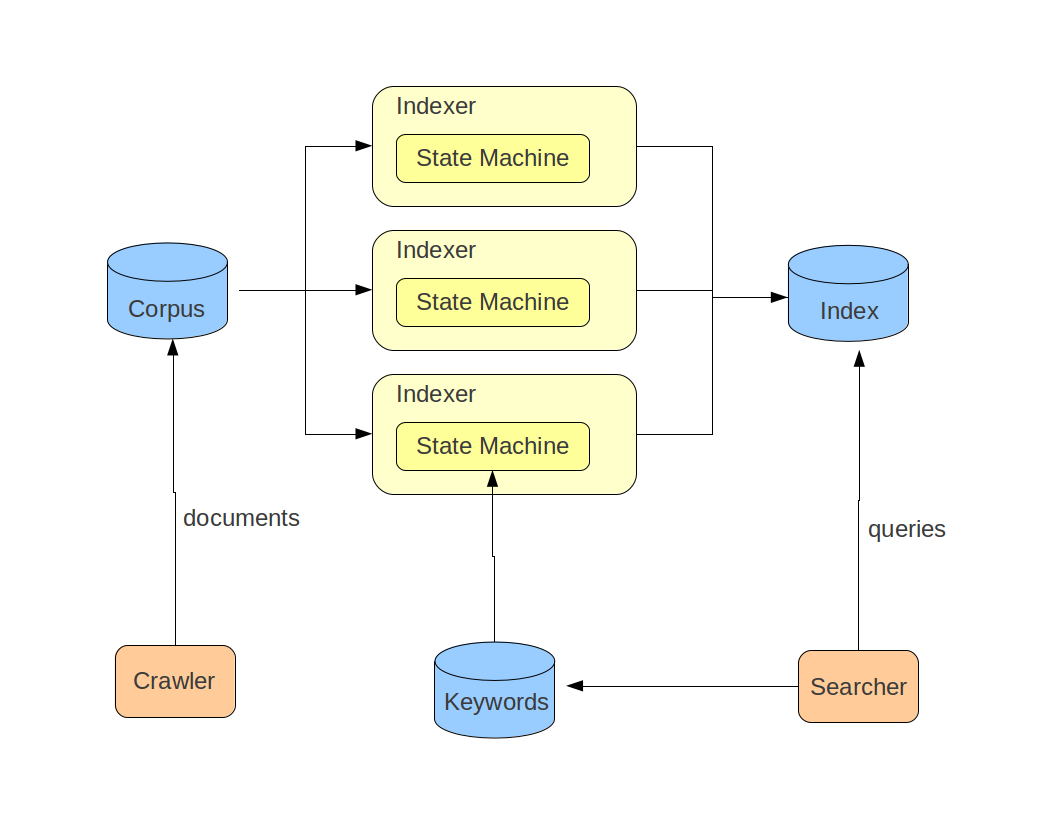
\includegraphics[width=\textwidth,height=!]{deploymentmodel}
  \end{center}
  \caption{Indexer deployment model}
  \label{fig:deploymentmodel}
\end{figure} 

A guiding architectural principal of the indexer design is to separate the implementation
into three logical layers:
\begin{itemize}
\item \textbf{Software Layer:} implements parsing, indexing and search
  algorithms.
\item \textbf{Data Access Layer:} implements an
  \textit{object-relational mapping}, insulating algorithm
  implementation from the persistence details. This layer implements
  classes which encapsulate persistent entities within the system.
\item \textbf{Database:} the persistent store for the document
  collection and inverted index.
\end{itemize}

The implementation classes and their relationships are represented in
a UML class diagram in figure \ref{fig:overallclassdiagram}. Figure
\ref{fig:overallsequencediagram} is a UML sequence diagram showing how
the layers interact at a high level.  The implementation of each of
these layers is described in more detail in section
\ref{sec:implementation}.

\begin{figure}
  \begin{center}
	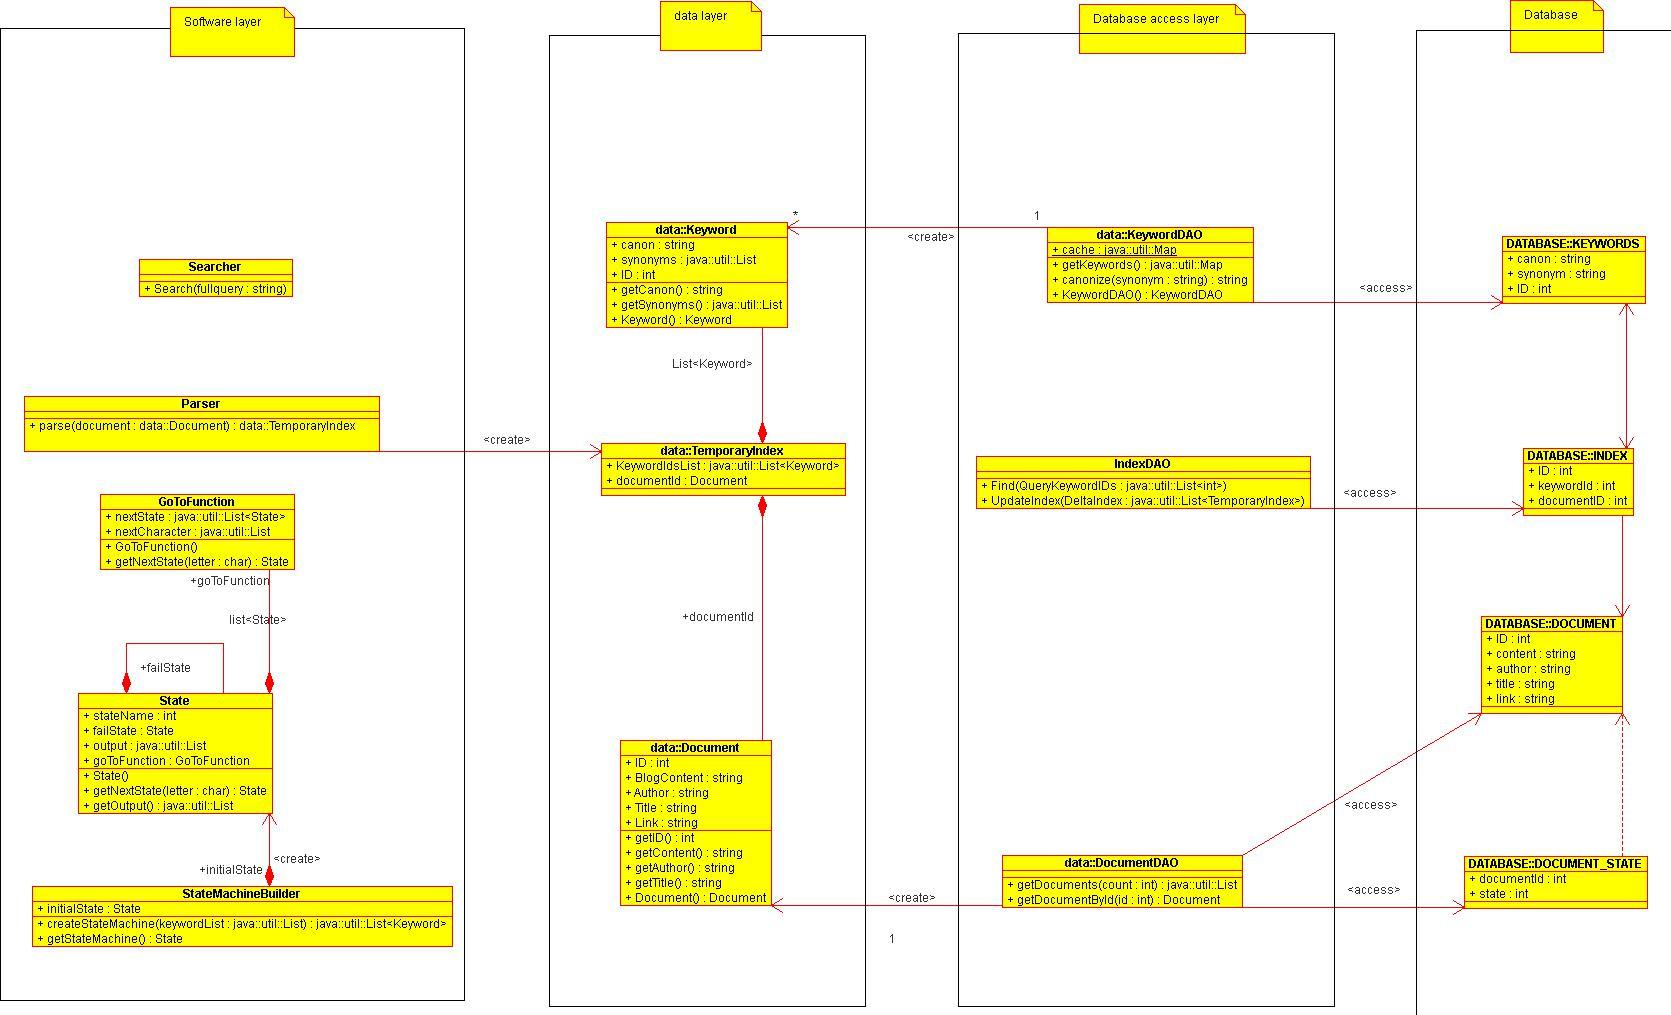
\includegraphics[width=\textwidth,height=!]{overallclassdiagram}
  \end{center}
  \caption{Overall UML class diagram design}
  \label{fig:overallclassdiagram}
\end{figure} 

\begin{figure}
  \begin{center}
	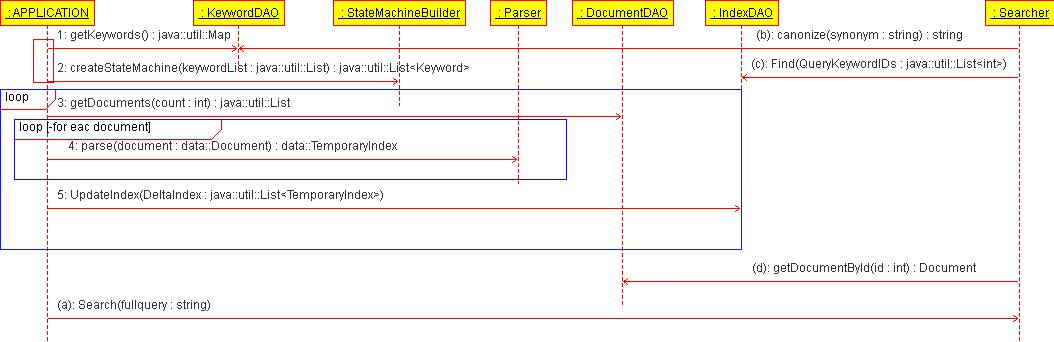
\includegraphics[width=\textwidth,height=!]{overallsequencediagram}
  \end{center}
  \caption{Overall UML sequence diagram design}
  \label{fig:overallsequencediagram}
\end{figure} 





%----------------------------------------
% Implementation 
%----------------------------------------
\section{Implementation}
\label{sec:implementation}
The individual worker processes of the indexer system are implemented as Java
programs. The programs make use of the following thirdparty libraries:

\begin{itemize}
  \item \textbf{DBPool:} a database connection pooling library, used
    to manage connections to relational databases.
  \item \textbf{Apache Commons Logging:} a generic logging API used by
    DBPool.
  \item \textbf{Apache Commons CLI:} a library for parsing command
    line arguments passed to Java programs.
  \item \textbf{MySQL JDBC driver:} the MySQL Java client driver.
\end{itemize}


The indexer system maintains an \textit{inverted index} of an evolving
corpus and services concurrent search requests against the index. The
current implementation is based on boolean retrieval methods described
in \cite{RefWorks:109}. An Aho-Corasick state machine
\cite{RefWorks:103} is used to scan documents for a predefined set of
keywords, and construct a term index for each document (delta
index). The term occurrences for each document are used to augment an
existing index for documents already processed. The document
collection, index, and keyword list are maintained in a single MySQL
database instance. It is through this database that the parallel
indexer instances are initialized and synchronized. This configuraion
is operationally simple and easy to implement but has the potential to
become a throttle point as the system is scaled to larger and
faster-evolving document collections, and is required to service a
higher rate of queries. In order to scale the current implementation
to large document collections, a more efficient mechanism would be
required in this repect.

The following subsections detail the implementation of the
architectural layers identified in section \ref{sec:designcomponent}.


\subsection{Data Access Layer}
\label{sec:dataaccesslayer}
Access to persistent storage is via objects of the data access
layer. Confining data access to a logical grouping of classes
insulates the other application components from changes in database
schema.


\subsubsection{Document}
\label{sec:document}
The DocumentDAO singleton class provides methods for retrieving
Document objects from the document database: List <Document>
getDocuments (int count): retrieve a specified number of unprocessed
documents from the database. The documents retrieved will be
atomically marked as processed so that processing is not duplicated on
other nodes. In this scheme, a document is considered processed to all
other processes once retrieved from the database. This may cause
problems from a fault recovery perspective if the processing node
fails. A proposed enhancement to this scheme is to use another state,
processing, to indicate that the document has been retrieved and to
update the state to a processed state once processing is actually
complete. For the initial implementation we will use the processed
state only.
Document getDocumentById (int id): retrieve a specific document from the database, referenced by its ID.
Int getID (): accessor method.
String getContent (): accessor method.
String getAuthor (): accessor method.
String getTitle (): accessor method
String getLink(): accessor method.

The Document class encapsulates the BLOG database table, with the
addition of a state field that tracks whether a document has been
processed or not. This field will be implemented as a new field on the
BLOG table or as a new reference table DOCUMENT_STATE.  and show UML
class and sequence diagrams respectively for non-trivial classes and
methods involved in the implementation of the Document data access
layer.


%----------------------------------------
% Experiment Results
%----------------------------------------
\section{Experiment Results}
\label{sec:experimentresults}
FIX: All tests were run on a Dell laptop with an Intel Core Duo 2GHz
processor, 1GB RAM, running a 32 bit Linux 2.6.37 kernel. The Java
Virtual Machine used was version 1.6.0-24. 


\subsection{Aho-Corasick}
Various tests were conducted to characterize the performance of the
Aho-Corasick search algorithm:

\begin{itemize}
\item The time taken to construct the Aho-Corasick state machine was
  measured for different numbers of keywords. The results of this test
  is shown in figure \ref{fig:ahostatemachine} and construction time
  can easily be considered linear with respect to the number of
  keywords. This is consistent with \cite{RefWorks:103} which proves
  that the state machine construction algorithm is linearly
  proportional to the sum of the lengths of the keywords used to
  construct the state machine.

\item The time taken for the Aho-Corasick state machine to scan
  different sized corpora was measured. The test was repeated for
  various state machines, constructed using a 100, 200, and 400
  keyword set. The results of this test are shown on figure
  \ref{fig:ahoscan} and indicate that scan time is nearly linear with
  respect to the size of the corpus and independent of the number of
  keywords used to generate the state machine. This last result is
  consistent with \cite{RefWorks:103} which proves that the number of
  state transitions involved in processing an input string is
  independent of the number of keywords used to construct the state
  machine.

\item The time taken to search for different numbers of keywords was
  measured over different sized corpora. A set of ten keywords was
  selected randomly and the the corpora searched for ${n \choose k}$
  enumerated combinations thereof to obtain an average for a
  particular keyword set size. The results of this test are shown in
  figure \ref{fig:ahosearch} and indicate that search time is
  independent of the number of terms used in the search and linear
  with respect to the size of the corpus. This first result is
  surprising given that the search process exists as soon as a single
  instance of each search term is found. One would expect the number
  of documents scanned completely to increase as the number of search
  term increases. The small average document size and the fact that
  the search hit rate is low may account for this phenomenon.
\end{itemize}


\begin{figure}
  \begin{center}
	\includegraphics[width=\textwidth,height=!]{ahostatemachine}
  \end{center}
  \caption{Aho-Corasick state machine construction}
  \label{fig:ahostatemachine}
\end{figure} 

\begin{figure}
  \begin{center}
	\includegraphics[width=\textwidth,height=!]{ahoscan}
  \end{center}
  \caption{Aho-Corasick state machine scanning}
  \label{fig:ahoscan}
\end{figure} 

\begin{figure}
  \begin{center}
	\includegraphics[width=\textwidth,height=!]{ahosearch}
  \end{center}
  \caption{Aho-Corasick state machine search}
  \label{fig:ahosearch}
\end{figure} 


\subsection*{Inverted Index}
Various tests were conducted to characterize the performance of the
inverted index search algorithm:

\begin{itemize}
\item The time taken to construct the inverted index was measured for
  different sized corpora. The results of this test is shown in figure
  \ref{fig:invscan} and, as expected, indicate a linear relationship
  between index construction time and the size of the corpora.

\item The time taken to search for different numbers of keywords was
  measured over different sized corpora. A set of ten keywords was
  selected randomly and the the corpora searched for ${n \choose k}$
  enumerated combinations thereof to obtain an average for a
  particular keyword set size. The results of this test are shown in
  figure \ref{fig:invsearch}. If the results for one and ten search
  words are ignored, search times appear to be independent of the
  number of search terms and close to linear with respect to the size
  of the corpus. The unusual results for one and ten keywords warrant
  further investigation.
\end{itemize}


\begin{figure}
  \begin{center}
	\includegraphics[width=\textwidth,height=!]{invscan}
  \end{center}
  \caption{Inverted index creation}
  \label{fig:invscan}
\end{figure} 

\begin{figure}
  \begin{center}
	\includegraphics[width=\textwidth,height=!]{invsearch}
  \end{center}
  \caption{Inverted index search}
  \label{fig:invsearch}
\end{figure} 


\subsection{Comparison}
Comparing corpus scan times for Aho-Corasick and inverted index
implementations, figures \ref{fig:ahoscan} and \ref{fig:invscan}
respectively, indicates that the inverted index scanner is
significantly faster than the Aho-Corasick state machine. Given that
the grammar supported by the JFlex-generated scanner is more expressive
than that of the Aho-Corasick state machine, one would expect results
to more comparable. Reviewing the source code of the generated scanner
indicates a compact and efficient implementation using packed data
structures to represent the internal state machine. In comparison, the
Aho-Corasick implementation is relatively unoptimized, closely
following the pseudo-code in \cite{RefWorks:103}.

Comparing search times for Aho-Corasick and inverted index
implementations, figures \ref{fig:ahosearch} and \ref{fig:invsearch}
respectively, indicates that the inverted index implementation has an
advantage of several orders of magnitude. The initial cost of creating
the inverted index is significantly larger than the creation of the
Aho-Corasick state machine however this cost is amortized over each
subsequent search. The Aho-Corasick implementation rescans the entire
corpus for each search, as opposed to a scan of the inverted index
alone. This exercise is a classic demonstration of the impetus behind
using indexed search techniques for large corpora.


%----------------------------------------
% Conclusions
%----------------------------------------
\section{Conclusions}
\label{sec:conclusions}


%----------------------------------------
% Bibliography
%----------------------------------------
% Change Bibliography title to 'References'
\renewcommand\refname{References}
\bibliography{bibliography}
\bibliographystyle{IEEEannot}


%--------------------------------------------------
\end{document}
